\section{Entropia Cruzada}

A \emph{entropia}\index{entropia!cruzada} cruzada é uma medida frequentemente utilizada para comparar duas
distribuições de probabilidade. Ela desempenha um papel importante em aprendizado de máquina.
Podemos interpretar a entropia cruzada como a ``surpreza'' da previsão feita por um modelo
em relação à verdadeira distribuição de probabilidades. 

O comprimento ótimo de um código para uma variável aleatória $X$ com
distribuição $p$ é dada pela entropia $H(X)$, ou seja, $H(p)$. Entretanto, se
$X$ for codificada com um código otimizado para uma distribuição $q$, o
comprimento esperado do código será dado pela entropia cruzada de $p$ e $q$:
\begin{subequations}
\begin{align}
\E_p [\ell] &= - \E_p [\log q(x)] \\
            &= - \sum_{x \in \mathcal{X}} p(x) \log q(x) .
\end{align}
\end{subequations}



\begin{definition}[Entropia Cruzada]
Seja $p = \{ p(x) \}_{x \in \mathcal{X}}$ uma distribuição de probabilidade
verdadeira e $q = \{ q(x) \}_{x \in \mathcal{X}}$ uma distribuição aproximada,
onde $\mathcal{X}$ é o alfabeto. A entropia cruzada entre $p$ e $q$ é definida
como:
\begin{equation}\label{eq:crossentropy}
H(p, q) = - \sum_{x \in \mathcal{X}} p(x) \log q(x) .
\end{equation}
\end{definition}

A entropia cruzada pode ser interpretada como o número esperado de bits
necessários para codificar eventos gerados pela distribuição verdadeira $p$,
utilizando um código otimizado para a distribuição aproximada $q$.
Intuitivamente, ela quantifica o ``custo'' de usar uma distribuição errada $q$
para modelar $p$.

\begin{proposition}
A entropia cruzada\index{entropia!cruzada, relação com divergência} está relacionada à entropia de $p$ e à divergência de
Kullback-Leibler (KL)\index{divergência de Kullback-Leibler!relação com entropia cruzada} entre $p$ e $q$. Especificamente:
\begin{equation}\label{eq:crossentropykldiv}
H(p, q) = H(p) + D_{\text{KL}}(p \| q),
\end{equation}
onde $H(p) = - \sum_{x \in \mathcal{X}} p(x) \log p(x)$ é a entropia de $p$ e 
$D_{\text{KL}}(p \| q) = \sum_{x \in \mathcal{X}} p(x) \log \frac{p(x)}{q(x)}$ 
é a divergência KL entre $p$ e $q$.
\end{proposition}

\begin{proof}
Escrevendo a entropia cruzada:
\begin{subequations}\label{eq:crossentropykldiv}
\begin{align}
H(p, q) &= - \sum_{x \in \mathcal{X}} p(x) \log q(x) \\
        &= \sum_{x \in \mathcal{X}} p(x) \log \frac{p(x)}{p(x)q(x)} \\
        &= \sum_{x \in \mathcal{X}} p(x) \log \frac{1}{p(x)} + \sum_{x \in \mathcal{X}} p(x) \log \frac{p(x)}{q(x)} \\
        &= H(p) + D(p\|q) .
\end{align}
\end{subequations}
\end{proof}

A \Cref{eq:crossentropykldiv} revela que a entropia cruzada é composta pela incerteza intrínseca de $p$ (i.e. $H(p)$)
e pela penalidade devido à diferença entre $p$ e $q$ (i.e. $D(p\|q)$). Como $D(p\|q) \geq 0$, segue que
\begin{equation}
H(p, q) \geq H(p),
\end{equation}
com igualdade se, e somente se, $p = q$. Nesse caso, quando o modelo $q$ é perfeito, 
a entropia cruzada reduz-se à entropia de $p$, pois $D(p\|q) = 0$. 
Assim, usar um modelo imperfeito nunca reduz a surpresa média em relação à distribuição verdadeira.

Outra característica da entropia cruzada é a assimetria: $H(p, q) \neq H(q, p)$. 
Isso reflete o fato de que os papéis de $p$ (distribuição verdadeira) e $q$ (modelo) não são intercambiáveis. 
Trocar $p$ e $q$ altera a interpretação, pois estaríamos codificando eventos de $q$ com um código 
otimizado para $p$, o que geralmente leva a resultados distintos.





\subsection{Aprendizado de Máquina}

Em aprendizado de máquina, a entropia cruzada é utilizada como uma
função de perda em problemas de classificação. Considere um problema de
classificação com $K$ classes, onde a distribuição verdadeira $p$ representa a
probabilidade real de cada classe (geralmente, uma distribuição degrau, com
$p(y_i) = 1$ para a classe correta $y_i$ e $0$ para as demais). Um modelo
preditivo, como uma rede neural, produz uma distribuição aproximada 
$q = \{q(y_i) \}_{i=1}^K$, onde $q(y_i)$ é a probabilidade prevista para a classe
$y_i$.

A função de perda de entropia cruzada, para uma única amostra com classe verdadeira $y_i$, é dada por:
\begin{equation}
L = - \log q(y_i).
\end{equation}
Para um conjunto de $N$ amostras, a perda média é:
\begin{equation}
L = - \frac{1}{N} \sum_{i=1}^N \log q(y_i).
\end{equation}
Essa perda é minimizada quando $q(y_i) \to 1$ para a classe correta, ou seja,
quando o modelo prediz corretamente a distribuição verdadeira. A minimização da
entropia cruzada equivale a minimizar a divergência KL entre $p$ e $q$, já que
$H(p)$ é constante para um conjunto de dados fixo.

\begin{example}
Em uma tarefa de classificação com três classes (``A'', ``B'', ``C''), 
suponha que a classe verdadeira seja ``A''. 
A distribuição verdadeira é $P = (1, 0, 0)$. 
Se o modelo prediz $Q = (0.7, 0.2, 0.1)$, a perda de entropia cruzada é:
\[
L = - \log 0.7 \approx 0.5146.
\]
Se o modelo melhorar sua predição para $Q = (0.9, 0.05, 0.05)$, a perda diminui para:
\[
L = - \log 0.9 \approx 0.1520.
\]
\end{example}

A entropia cruzada é particularmente eficaz em aprendizado de máquina porque
fornece um gradiente bem definido para otimização, permitindo que algoritmos
como gradiente descendente ajustem os parâmetros do modelo de forma eficiente.
Além disso, sua interpretação em termos de teoria da informação conecta
diretamente o treinamento de modelos à ideia de redução de incerteza sobre a
distribuição verdadeira.


% verificar e melhorar
%\begin{example}
%No problema de classificação de vinhos do repositório UCI, com três classes de
%cultivares, considere um modelo de regressão softmax com pesos 
%$w_1, w_2, w_3 \in \mathbb{R}^{13}$ e vieses $b_1, b_2, b_3$ para as três classes, utilizando
%13 características (e.g., álcool, ácido málico). Para uma amostra da classe
%``Cultivar 1'' com características $x \in \mathbb{R}^{13}$ (padronizadas) e
%rótulo verdadeiro $y = (1, 0, 0)$, as probabilidades são:
%\[
%q_i = \frac{e^{w_i \cdot x + b_i}}{e^{w_1 \cdot x + b_1} + e^{w_2 \cdot x + b_2} + e^{w_3 \cdot x + b_3}}, \quad i = 1, 2, 3.
%\]
%Para um modelo inicial com $w_1 = (-2, -2, \ldots)$, $w_2, w_3$ fixos e $b_i = 0$, 
%obtemos probabilidades aproximadas $q \approx (0.7, 0.2, 0.1)$, com perda
%de entropia cruzada:
%\[
%L = - \log q_1 \approx 0.357.
%\]
%Após 50 iterações de gradiente descendente com taxa de aprendizado 
%$\eta = 0.1$, os pesos são ajustados, resultando em $q \approx (0.9, 0.05, 0.05)$ e uma
%perda menor:
%\[
%L = - \log 0.9 \approx 0.105.
%\]
%O mesmo processo aplica-se a amostras das classes ``Cultivar 2'' ($y = (0, 1, 0)$) e ``Cultivar 3'' ($y = (0, 0, 1)$). 
%A \Cref{fig:cross_entropy_contours} mostra três superfícies de perda,
%uma para cada classe, em função dos pesos $w_{i1}$ (álcool) e $w_{i2}$ (ácido
%málico) de cada classe, com a trajetória de gradiente descendente indicando a
%minimização da entropia cruzada.
%
%\begin{figure}[ht]
%\centering
%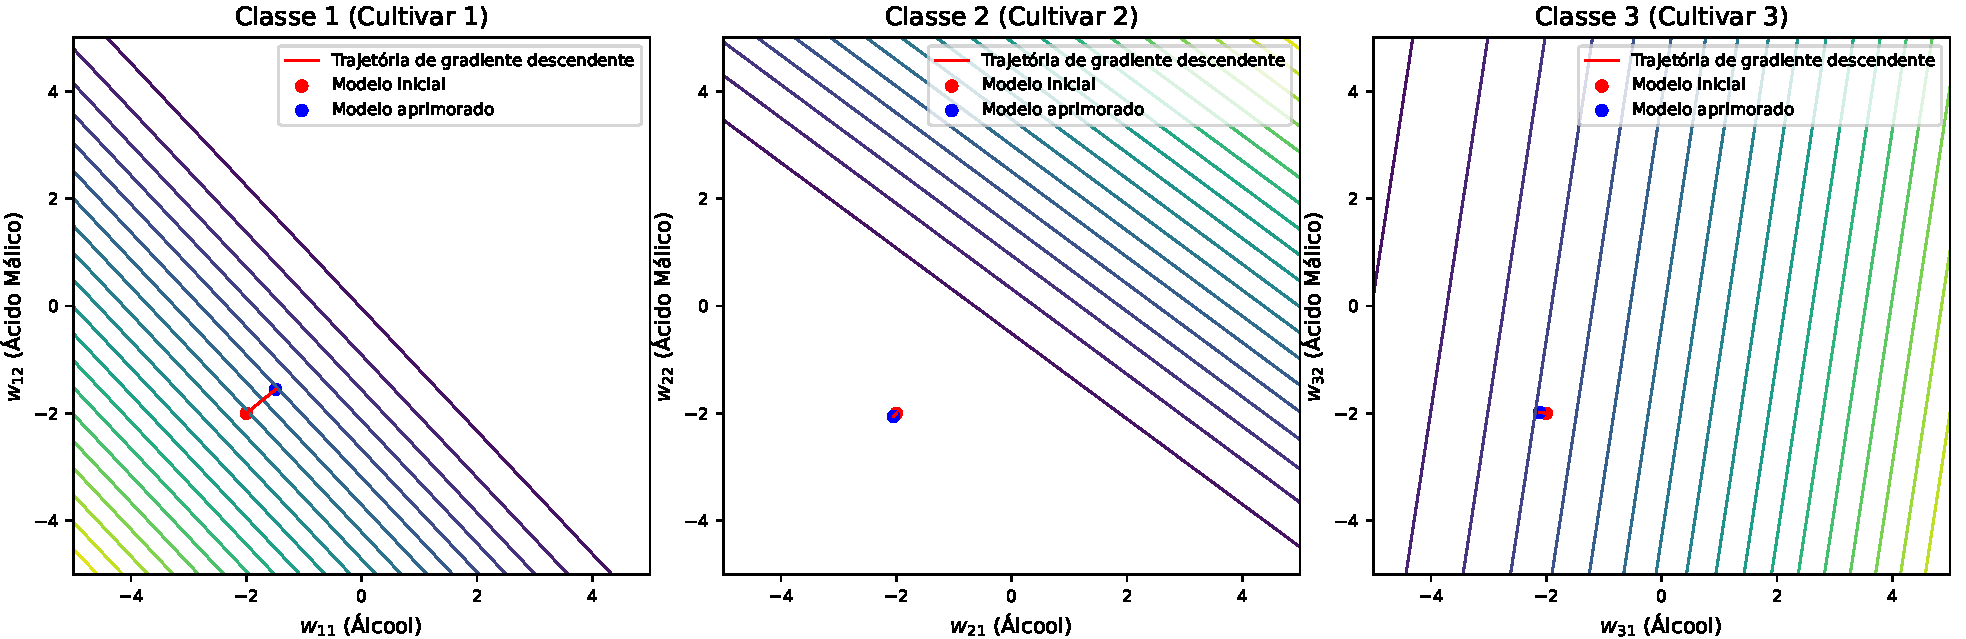
\includegraphics[width=\textwidth]{figures/cross_entropy_contours.pdf}
%\caption{Curvas de contorno da perda de entropia cruzada para uma amostra de
%cada classe do conjunto de vinhos UCI. Cada subfigura mostra a perda em função
%dos pesos $w_{i1}$ (álcool) e $w_{i2}$ (ácido málico) para a classe $i$, com a
%trajetória de gradiente descendente (linha vermelha). Os pontos vermelhos
%indicam o modelo inicial e os pontos azuis indicam o modelo aprimorado.}
%\label{fig:cross_entropy_contours}
%\end{figure}
%
%\end{example}
